\documentclass[dvipsnames,mathserif]{beamer}
\setbeamertemplate{footline}[frame number]
%\setbeamertemplate{itemize/enumerate body begin}{\large}
%\setbeamertemplate{itemize/enumerate subbody begin}{\large}
\setbeamercolor{footline}{fg=black}
\setbeamerfont{footline}{series=\bfseries}
\usepackage{tikz}
\usepackage{xcolor}
\usepackage{graphicx, setspace, appendix, mathrsfs, amsmath, amsfonts,caption, mathtools}
\usepackage[english]{babel}
%\usetheme{Frankfurt}%1
\usetheme{Darmstadt}%1

% for RTL liste
\makeatletter
\newcommand{\RTListe}{\raggedleft\rightskip\leftm}
\newcommand{\leftm}{\@totalleftmargin}
\newcommand{\rnumber}[1]{\uppercase\expandafter{\romannumeral #1\relax}}
\makeatother

% RTL frame title
\setbeamertemplate{frametitle}
{\vspace*{-1mm}
  \nointerlineskip
    \begin{beamercolorbox}[sep=0.3cm,ht=2.2em,wd=\paperwidth]{frametitle}
        \vbox{}\vskip-2ex%
        \strut\hskip1ex\insertframetitle\strut
        \vskip-0.8ex%
    \end{beamercolorbox}
}
% align subsection in toc
\makeatletter
\setbeamertemplate{subsection in toc}
{\leavevmode\rightskip=5ex%
  \llap{\raise0.1ex\beamer@usesphere{subsection number projected}{bigsphere}\kern1ex}%
  \inserttocsubsection\par%
}
\makeatother

% RTL triangle for itemize
\setbeamertemplate{itemize item}{\scriptsize\raise1.25pt\hbox{\donotcoloroutermaths$\blacktriangleleft$}} 

%\setbeamertemplate{itemize item}{\rule{4pt}{4pt}}

\defbeamertemplate{enumerate item}{square2}
{\LR{
    %
    \hbox{%
    \usebeamerfont*{item projected}%
    \usebeamercolor[bg]{item projected}%
    \vrule width2.25ex height1.85ex depth.4ex%
    \hskip-2.25ex%
    \hbox to2.25ex{%
      \hfil%
      {\color{fg}\insertenumlabel}%
      \hfil}%
  }%
}}

\setbeamertemplate{enumerate item}[square2]
\setbeamertemplate{navigation symbols}{}


\titlegraphic { 
\begin{tikzpicture}[overlay,remember picture, opacity=0.1,]
\node[] at (0, 2.9){
};\end{tikzpicture}}
\setbeamertemplate{caption}[numbered]
\begin{document}

\rightskip\rightmargin
\title{Exploiting Symmetry in High-Dimensional Dynamic Programming}
\author{Mahdi Ebrahimi Kahou, Jesús Fernández-Villaverde, Jesse Perla and Arnav Sood}

\institute{Boston College}
\footnotesize{\date{\today }


\begin{frame}
\maketitle
\end{frame}


%
\footnotesize \tableofcontents
%
\section{Introduction}
\begin{frame}{Introduction}
    \begin{itemize}
        \item A new method for solving high-dimensional dynamic programming problems with a finite but large number of heterogeneous agents. Accurate and quick.\\
        \vspace{0.2cm}
        \item Permutation invariance.
        \vspace{0.2cm}
        \item Concentration of measure.
        \vspace{0.2cm}
        \item Design and train deep learning architectures that exploit symmetry and concentration of measure.
        \item Use multi-firm investment under uncertainty model to demenstrate the performance of the method. 
    \end{itemize}
\end{frame}


\section{Permutation Invariance}
\begin{frame}{Permutation Invariance}
    \begin{itemize}
        \item Exploit symmetry in the solution of dynamic programming problems to reduce dimensionality.\\
        \vspace{0.2cm}
        \item Permutation-invariant function:
        \[f(x,\pi X) = f(x,X)\]
        $\pi$ is a $N$-dimensional permutation matrix
        %\item Dynamic programming\\
        %\begin{align*}
        %v(x,X) &= \underset{u}{max}\{r(x,u,X) + \beta E[v(x',X')]\}\\
        %s.t.\, x' &= g(x,u) + \sigma w + \eta \omega\\
        %X'&= G(X) + \Omega W + \eta\omega\bf{1}_{N}
        %\end{align*}
        %\item Permutation invariance:
        %\begin{align*}
        %&r(x,u,\pi X) = r(x,u,X),\,G(\pi X) = \pi G(X),\,\pi \Omega = \Omega \pi \\
        %&\Rightarrow \; u(x,\pi X) = u(x,X),\,v(x,\pi X) = v(x,X)
        %\end{align*}
        \item Proposition 2: Representation of permutation-invariant functions
        \begin{align*}
        &f(x,X) = \rho(x,\frac{1}{N}\sum_{i=1}^{N}\phi(X_i))\\
        &\rho: R^{L+1} \rightarrow R ,\; \phi: R \rightarrow R^{L}
        \end{align*}
        \item How to exploit it?
    \end{itemize}
\end{frame}


\section{Concentration of Measure}
\begin{frame}{Concentration of Measure}
    \begin{itemize}
        \item Can calculate high-dimensional expectations using single Monte Carlo draw.\\ 
        \vspace{0.1cm}
        \item Proposition 3: Concentration of measure when expected gradients are bounded in N
        \begin{align*}
        P(|f(z^1) - E[f(z)]| \geq \epsilon) \leq \frac{\rho(\Sigma)}{\epsilon^2}\frac{1}{N}
        \end{align*}
        Provide an upper bound on the error of the evaluation of the expectation. 
        It is usually better to approximate $E [f (z)]$ by $f (z^1)$ than by $f(\bf{0}_N)$
        \vspace{0.2cm}
        \item How to exploit it?
    \end{itemize}
\end{frame}

\section{Model}
\begin{frame}{Model}
Investment under uncertainty with many firms:\\
    \begin{align*}
    v(x,X) & = \underset{u}{max}\;{p(X)x - \frac{\gamma}{2}u^2 + \beta E[v(x',X')]}\\
    s.t. \, x'&= (1-\delta)x + u + \sigma w + \eta \omega\\
    X'_{i} &= (1-\delta)X_{i} + \hat{u}(X_{i},X) + \sigma W_{i} + \eta \omega, \; for \, i\in\{2,...,N\}\\
    X'_1 &= (1-\delta)X_1 + \hat{u}(X_1,X) + \sigma w + \eta \omega
    \end{align*}
    where $p(X)$ (the inverse demand function) is assumed to be: \[p(X) = \alpha_0 - \alpha_1\frac{1}{N}\sum_{i=1}^{N}x_i^{\nu}\]
%Model solution: the Euler eqation
%\[\gamma u(x,X) = \beta E[P(X') + \gamma (1-\delta)u(x',X')]\]
%\[X' = \{(1-\delta)\hat{x} + u(\hat{x},X) + \sigma \hat{w} + \eta \omega,\; for \: (\hat{x},\hat{w}) \in (X,W)\}\]
\end{frame}

\section{Deep Learning}
\begin{frame}{Deep Learning}
    \begin{itemize}
        \item Approximate $\rho$, $\phi$ and $L$ using a deep learning architecture $F(\theta)$.
        \[u(x,X) = \rho(x,\frac{1}{N}\sum_{i=1}^{N}\phi(X_i))\]
        Networks: $\phi(Identity)$, $\phi(Moments)$ and $\phi(ReLU)$ with two layers each with 128 nodes (baseline case). 49.2K, 49.8K, and 66.8K parameters respectively, regardless of N.\\
        $\rho$ is approximated by networks with four layers each with 128 nodes.
        \vspace{0.1cm}
        \item Train the network by minimizing the Euler residuals:
        \[\varepsilon(x,X;\theta) \equiv \gamma u(x,X;\theta) - \beta E[P(X') + \gamma (1-\delta)u(x',X';\theta)]\]
        %$\Rightarrow$Pick ${X_m(0), ..., X_m(T )}$ for $m = 1, .., M$ trajectories given some initial points \\$\Rightarrow$ Evaluate $\varepsilon_{m,t}(x, X; \theta)$  \\$\Rightarrow$ Slove $\underset{\theta}{min}\frac{1}{M}\sum_{m=1}^{M}\sum_{t=0}^{T}(\varepsilon_{m,t}(x,X;\theta))^2$
    \end{itemize}
\end{frame}



\begin{frame}{Deep Learning}
Case I: $\nu = 1$\\
Analytical solution: $u(X) = H_0 + \frac{1}{N}H_1\sum_{i=1}^{N}x_i$
\begin{figure}[h!]
\centering
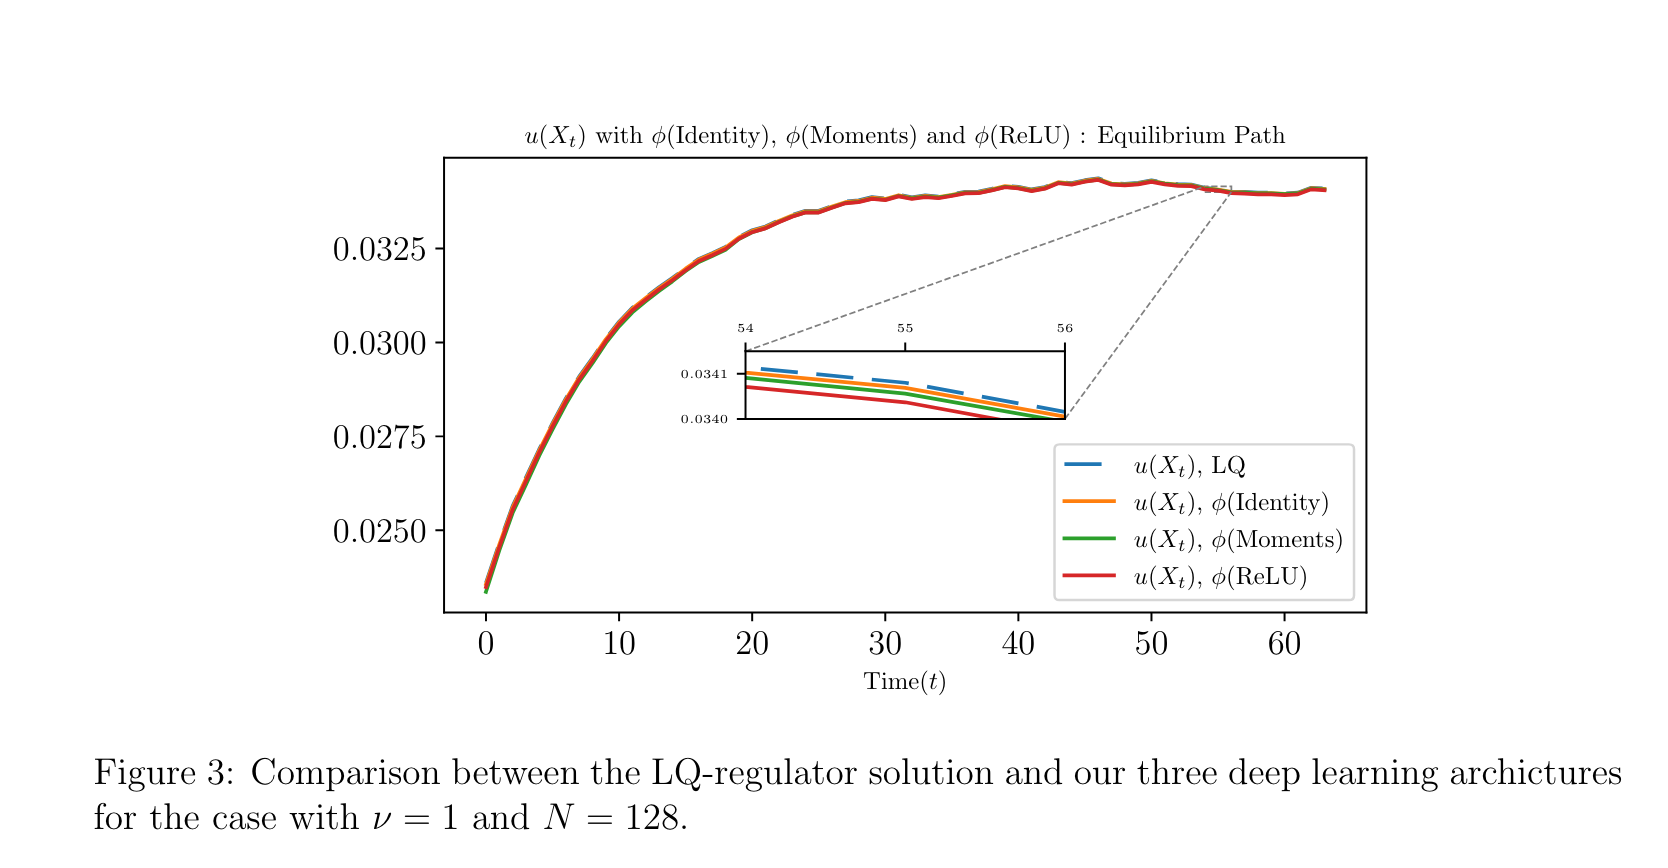
\includegraphics[width = 1.1\textwidth]{3.png}
\end{figure}
\end{frame}

\begin{frame}{Deep Learning}
Accuracy of the approximation:
\begin{figure}[h!]
\centering
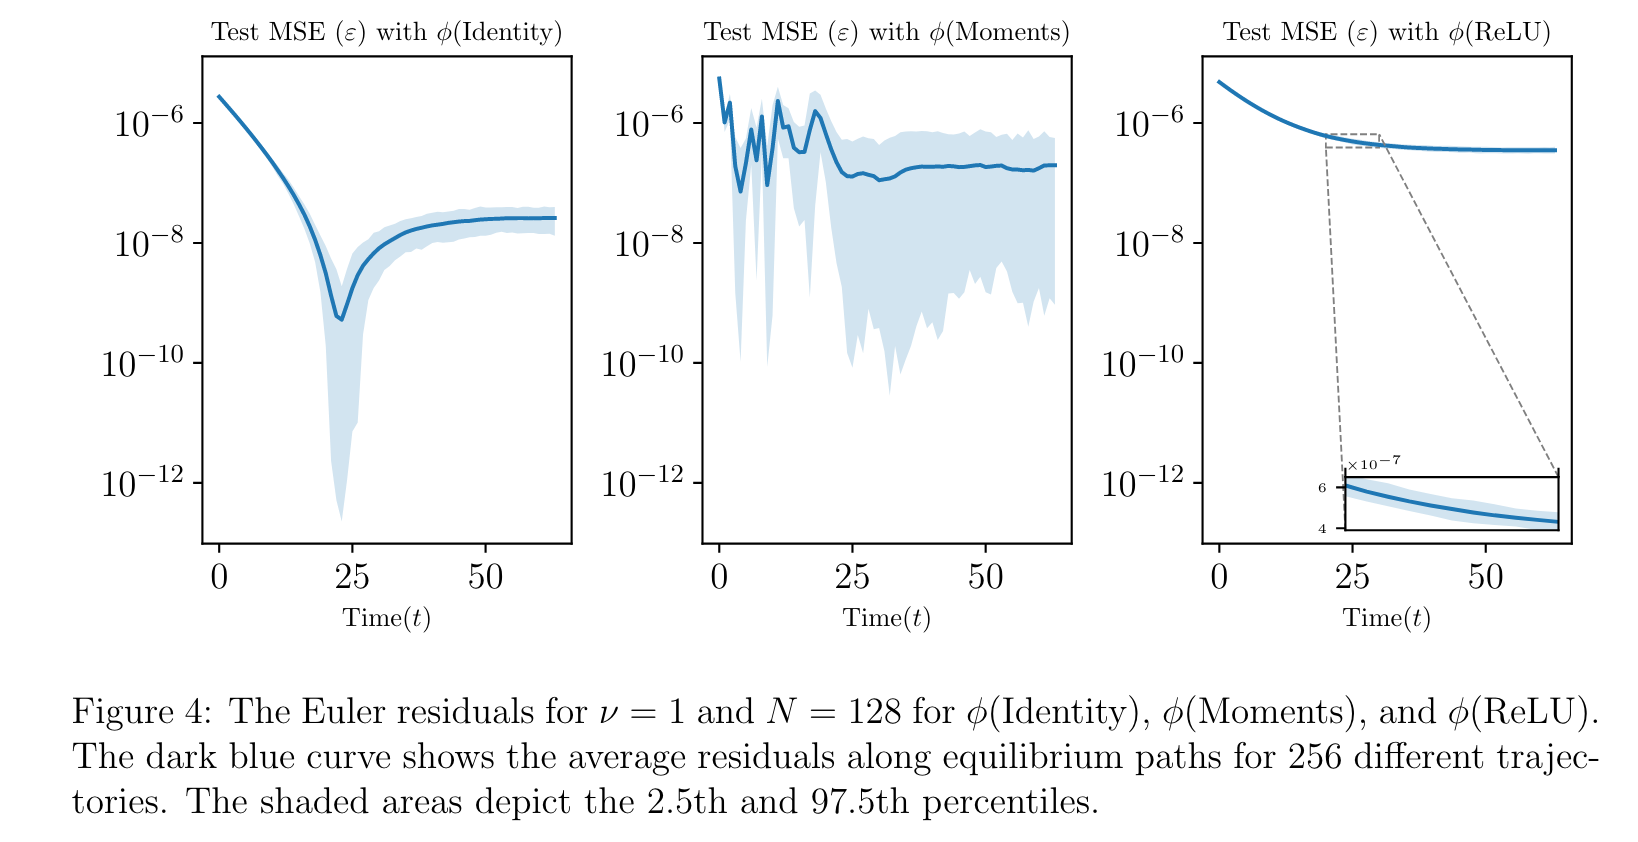
\includegraphics[width = 0.9\textwidth]{4.png}
\end{figure}
The ReLU architecture is especially stable. The extra parameters of this architecture help the function to generalize very consistently.
\end{frame}

\begin{frame}{Deep Learning}
Is it practical to implement?
\begin{figure}[h!]
\centering
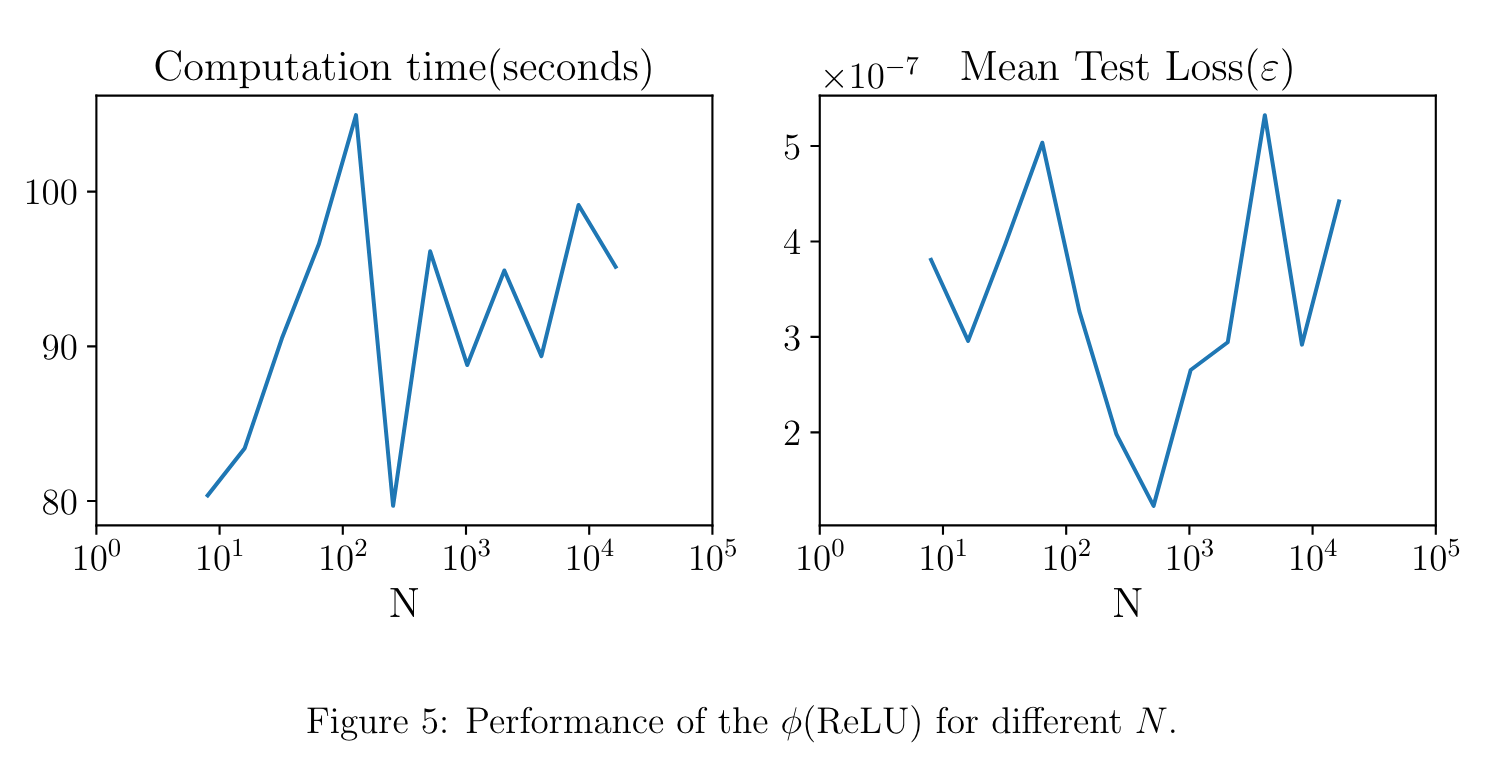
\includegraphics[width = 0.8\textwidth]{5.png}
\end{figure}
Computation time: of order $O(1)$ for reasonable N.
\end{frame}

\begin{frame}{Deep Learning}
Explore with different network architectures:
\begin{figure}[h!]
\centering
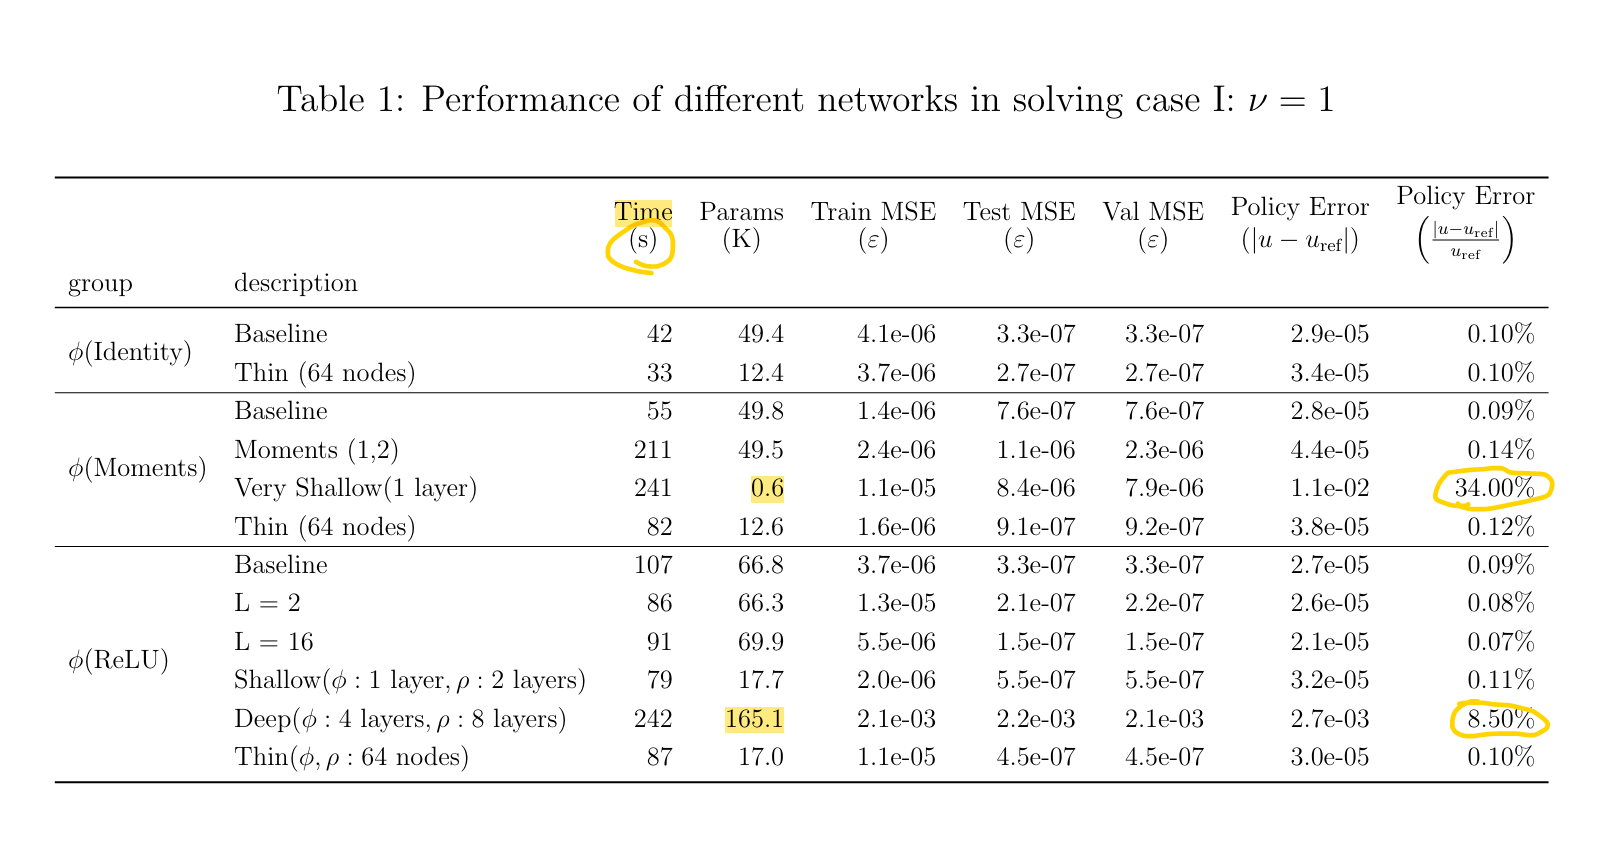
\includegraphics[width = 0.9\textwidth]{6.png}
\end{figure}
\begin{itemize}
    \item Very shallow in $\phi(Moments)$ finds a local minimum. Deep in $\phi(ReLU)$ is unsatisfactory. Explore different architectures.\\
    \item Results are better when we use a higher dimension of $L$.
\end{itemize}

\end{frame}

\begin{frame}{Deep Learning}
Case II: $\nu > 1$\\
No analytical solution.
\begin{figure}[h!]
\centering
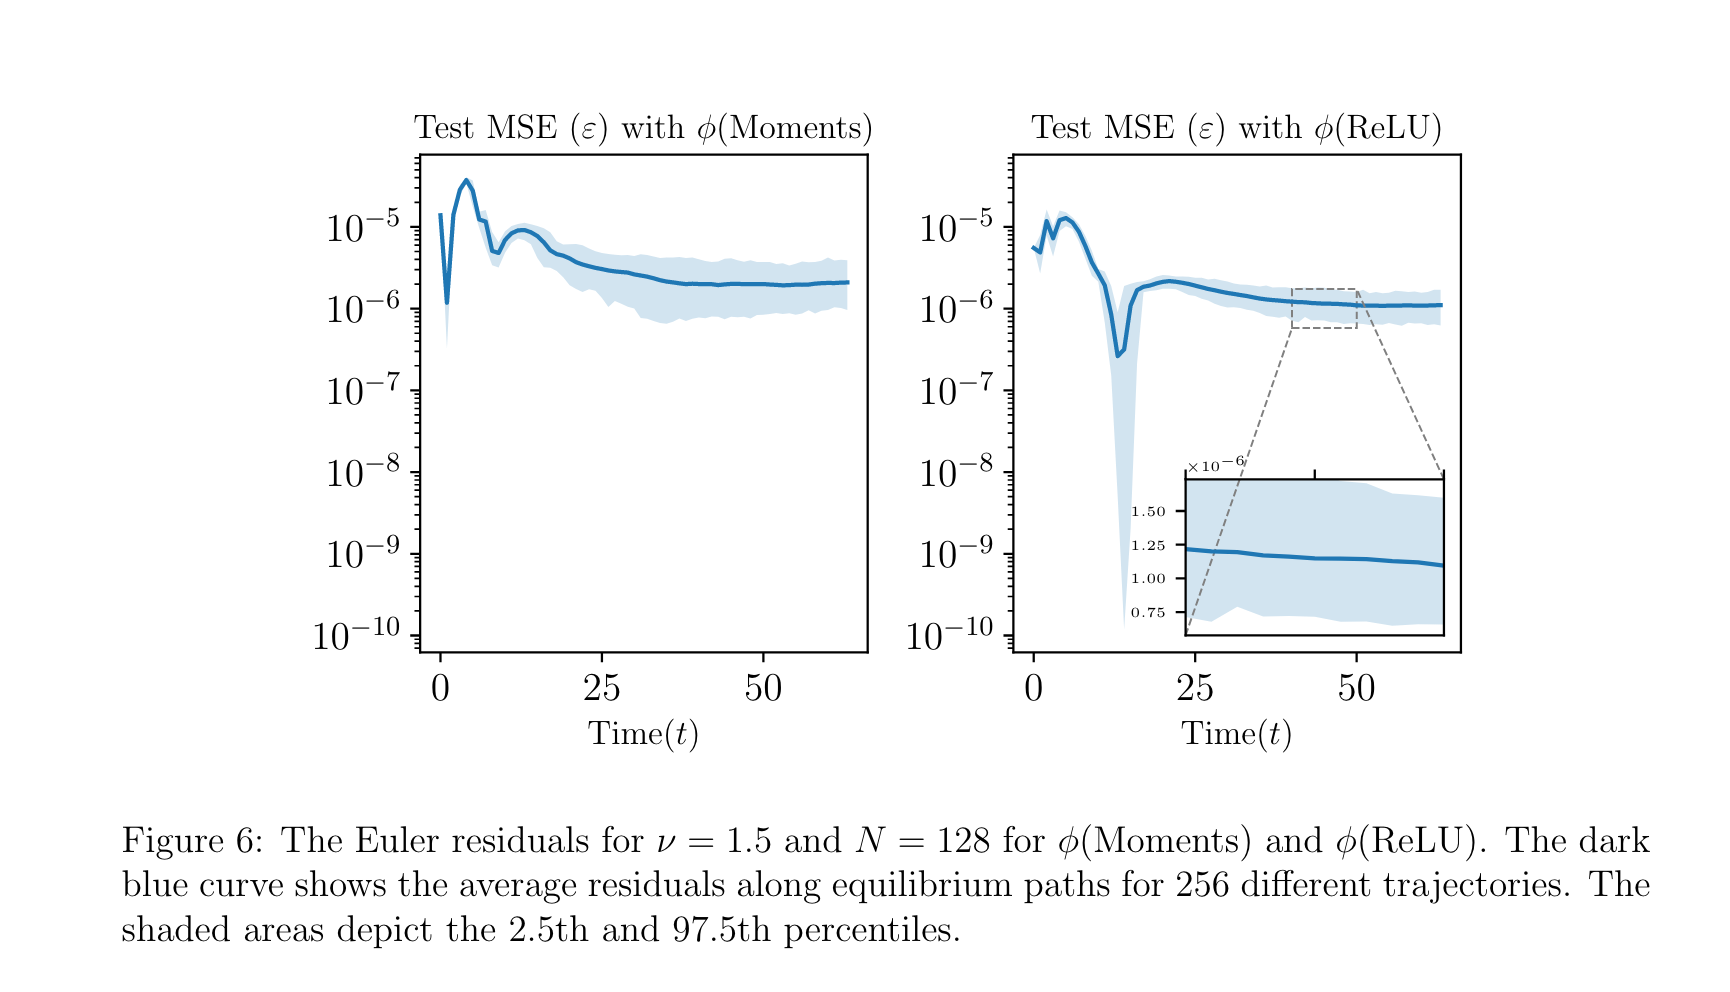
\includegraphics[width = \textwidth]{7.png}
\end{figure}
\end{frame}

\section{Extensions}
\begin{frame}{Extensions}
The tools are useful for solving any high-dimensional functional equations with some degree of symmetry, especially when these equations contain high-dimensional expectations.
    \begin{itemize}
        \item Decreasing returns to scale\\
        \vspace{0.2cm}
        \item Multiple productivity types\\
        \vspace{0.2cm}
        \item Complex idiosyncratic states\\
        \vspace{0.2cm}
        \item Global solutions with transitions and aggregate shocks

    \end{itemize}
\end{frame}

\section{Discussion}
\begin{frame}{Discussion}
    \begin{itemize}
        \item Solve high-dimensional dynamic programming problems in minutes.
        \vspace{0.2cm}
        \item Double-descent: by increase the number of parameters, we can both fit the data perfectly and achieve outstanding generalization.
        \vspace{0.2cm}
        \item Model selection since results are sensitive to different network architectures. 
    \end{itemize}
\end{frame}
\end{document}